% Lab 2 LaTeX Document
% Version 1.0
\documentclass{article}
\usepackage{listings}
\usepackage[margin=1in]{geometry}
\usepackage{graphicx}
\usepackage{textcomp}
%\usepackage{xcolor,colortbl}
\usepackage[table]{xcolor}
\usepackage{longtable}
\usepackage{caption}
\usepackage{fancyvrb}
\usepackage{placeins}
\usepackage[pdftex,
            pdfauthor={Paul Fortier, Daniel Noyes},
            pdftitle={Project Lab \#1 - Spring 2015 },
            pdfsubject={ECE 368 Digital Design},
            pdfkeywords={Digital Design, VHDL, Nexys 2, Xilinx, ISE},
            pdfproducer={Latex},
            pdfcreator={pdflatex}]{hyperref}


\captionsetup[table]{justification=centering}

%Remove the number display for each section tag
\makeatletter
\renewcommand\@seccntformat[1]{}
\makeatother

%Define gray center for a table
\definecolor{Gray}{gray}{0.85}
\newcolumntype{g}{>{\columncolor{Gray}}c}
%Quick command for multiple lines in a table cell
\newcommand{\specialcell}[2][c]{%
  \begin{tabular}[#1]{@{}c@{}}#2\end{tabular}}


\begin{document}

\begin{center}
\textsc{\huge ECE 368 Digital Design - Spring 2015}\\[1cm]
\textsc{{\LARGE Project Lab \#1: (100pts)}}\\[0.5cm]
\textsc{\Large Lab date: March $4$\textsuperscript{th} and March $11$\textsuperscript{th},2015}\\[0.5cm]
\textsc{\Large Lab Report Due: Wednesday March $25$\textsuperscript{th},2015}\\[1cm]
\end{center}

\section{Overview and Objectives:}
In this project assignment, you will be using the Xilinx ISE software tools with the Digilent Nexys 2 devboard to build the first part of your machine. You will be applying the experience you gained in the introduction labs in order to test your newly created hardware.

\section{Introduction to the UMD RISC}
In Figure~\ref{fig:pipetoplevel} below, it shows the top-level design connection a Control entity to an FPU entity. The FPU entity will expand upon the design experience you gained in Lab 2. The FPU will automatically run a program from the Control entity which is stored in the Instruction Memory entity. The Instruction Memory for now should hold up to 20 instructions through a five-stage pipeline and output the results from the NEXYS2 dev board to the VGA console. The Data Memory portion of the design and instruction set will only be used for the load word and store word instructions for this lab.

\begin{figure}[!htbp]
  \centering
    \fbox{\includegraphics[width=0.7\textwidth]{images/piplined_toplevel.png}}
  \caption{UMD RISC16 - Pipelined ALU Top-Level}
  \label{fig:pipetoplevel}
\end{figure}
\FloatBarrier

You will implement a full 5 cycle pipeline that takes in one instruction per clock cycle and performs partial operations on five instructions in parallel when the pipe is full. A full pipeline implies that there are 5 different instructions being performed, with each one in a different stage of the pipeline (i.e. one in fetch, decode, operand access, execution and write back). For the data path portion of this design you must implement the major elements of the Harvard Architecture. This includes the Instruction Memory, the Data memory, the functional processing unit (consisting of an arithmetic, logic, shift and load store unit), the sixteen 16 bit register bank and any other needed components. For example a program counter, instruction register, temporary registers and connecting devices (e.g. multiplexers, etc.). 

Table~\ref{tab:riscise} shows the instruction set architecture (ISA) you are to implement this in your machine. This portion of the instruction set includes the register type, immediate type, and data type instructions. You will need a variety of hardware components to implement these instructions.

\begin{table}[!htbp]
\rowcolors{2}{gray!25}{white}
  \begin{center}
    \begin{tabular}{|c|l|l|}
       \hline
       \rowcolor{gray!50}
       \large{\textbf{OPCODES:}} & \large{\textbf{Operation:}} & \large{\textbf{Routine:}} \\
       \hline 
       \textbf{0000} & ADD  REG A, REG B & R[A] $\leftarrow$ R[A] + R[B] set status flags NZVC  \\
       \textbf{0001} & SUB  REG A, REG B & R[A] $\leftarrow$ R[A] - R[B] set status flags NZVC  \\
       \textbf{0010} & AND  REG A, REG B & R[A] $\leftarrow$ R[A] \& R[B] set status flags NZVC  \\
       \textbf{0011} & OR   REG A, REG B & R[A] $\leftarrow$ R[A] $\mid$ R[B] set status flags NZVC  \\
       \textbf{0100} & MOV  REG A, REG B & R[A] $\leftarrow$ R[B] \\
       \textbf{0101} & ADDI REG A, IMMED & R[A] $\leftarrow$ R[A] + IMMED set status flags NZVC  \\
       \textbf{0110} & ANDI REG A, IMMED & R[A] $\leftarrow$ R[A] \& IMMED set status flags NZVC  \\
       \textbf{0111} & SL   REG A, IMMED[0..3] & R[A] $\leftarrow$  R[A\textless \textless IMMED] zero fill LSB C and V affected  \\
       \textbf{1000} & SR   REG A, IMMED[0..3] & R[A] $\leftarrow$ R[A\textgreater \textgreater IMMED] zero fill MSB  \\
       \textbf{1001} & LW   REG A, IMMED[7..0] & R[A] $\leftarrow$ MEM[IMMED]  \\
       \textbf{1010} & SW   REG A, IMMED[7..0] & MEM[IMMED] $\leftarrow$ R[A]  \\
       \hline
    \end{tabular}
  \end{center}
  \caption{UMD RISC-16 Partial Instruction Set Architecture (R, I, D type instructions)}
  \label{tab:riscise}
\end{table}
\FloatBarrier

A high level (not complete) notional design is depicted in Figure~\ref{fig:data_control_paths}. The clock, reset and other possibly needed control signals are implied in this design for readability. You will need to decide how you will clock devices, possibly even if you will clock them at all.

This lab introduces design decisions in creating and linking different combinational, behavioral and structural components together to work properly in a larger design. Pay careful attention to timing between different components and instructions in different phases of operation (fetch, decode, etc), Figure~\ref{fig:iec} and Figure~\ref{fig:pipeline_instruction_execution_example}.

For example, if you are reading in a new instruction value it must be stored in a register in order to stay stable, likewise every value must be stable before a write occurs. This can be ensured by performing writes during the next cycle or on an edge transitions. Although your design may work in simulation, you will find that the hardware is not as stable and predictable as you would expect. It will take a well laid out RTL designs, timing designs and test procedures to verify and validate your designs. Be precise and well organized. Lay out timing and control signal transitions carefully for each clock cycle to completely develop a working design.

\begin{figure}[!htbp]
  \centering
    \fbox{\includegraphics[width=0.5\textwidth]{images/iec.png}}
  \caption{Typical Instruction Execution Cycle}
  \label{fig:iec}
\end{figure}

\begin{figure}[!htbp]
  \centering
    \fbox{\includegraphics[width=0.5\textwidth]{images/pipeline_instruction_execution_example.png}}
  \caption{Concept for Pipelined Instruction Parallel Execution steps}
  \label{fig:pipeline_instruction_execution_example}
\end{figure}

\section{Procedure:}

\begin{enumerate}
% Part 1
  \item Complete the design of the Control Path entity. For this and later labs, this will be the center of your machine. This entity currently consists of possibly the following main components which must be implemented as separate VHDL entities, then integrated into the larger control entity:
  \begin{itemize}
    \item \textbf{Program Counter}: Controls the current instruction to be executed. Automatically increments on each clock cycle once started.
    \item \textbf{Pipeline Registers}: Multiple 16-bit registers must be created to hold instruction words (and state) for the appropriate pipeline stage.
    \item \textbf{Pipeline Controller}: Facilitates transition of instruction words for each pipeline cycle. Although we only have a few pipeline registers for now, this will be a great help once more stages are added and more sophisticated transitions are required.
    \item \textbf{Control Modules}: Act on the control signals based on the current instruction in the pipeline register for their associated pipeline stage. (i.e. CTRL1 acts on T1, CTRL2 acts on T2). These modules dictate the functionality of the rest of the machine. For example, if your current instruction is a register add, the control modules will decode the instruction to output the control signals for which register to read from, the operation to be performed, the logical flow of data through your FPU, and ultimately where to store it and when to enable the write enable back into the register bank and any other pertinent control signals.
  \end{itemize}
  Capture RTL diagrams of your design for your lab report.

% Part 2
  \item Create a testbench for your Control entity and verify its outputs are what you expect. Show that each instruction is read sequentially and propagated through pipeline. Verify and show that the control and data signals match your intended design.
  
  Document your test procedure, print your testbench results, and discuss any problems for your lab report.

% Part 3
  \item Construct the FPU entity and associated components. This design builds upon the ALU you experienced in Lab 1. For your reference, a sample design has been included in the class directory along with a testbench. If you decide to use some of these design concepts ensure that they fit your design and modify the entities and testbench as necessary.
  
  There are several components that must be wrapped around your ALU design. These are controlled by the control modules discussed in Step 1. Some notable entities are discussed as follows:
  
  \begin{itemize}
    \item \textbf{General Purpose Register Bank}: sixteen 16-bit general purpose registers (R0-R15). Similar in structure to the Instruction Memory in the Control entity except it is dual ported. You will have two address inputs, of which only will be written to from the data in din. Both outputs will reference the 16-bit register indexed by the two corresponding addresses.
    \item \textbf{Shadow Register Bank}: (SR0-SR3) for stack operations, and fast-interrupts supporting I/O operations. Implement but do not worry about implementing in your full architecture just yet.
    \item \textbf{Instruction Memory}: Read-only register containing 32, 16-bit words indexed by the address output from the program counter. Create this as a simple VHDL entity and initialize with your desired instruction word values. Since we are only accessing up to 20 instruction words for now, only the least significant five bits of the program counter are needed for instruction memory addressing. Figure~\ref{fig:instruction_format} shows the format of these instructions. You must correctly populate each field depending on the type of instruction you are executing and the desired output.
    \item \textbf{Data Memory}: Read-Write memory containing M, 16-bit words indexed by the address output from the instruction register. Create this as a VHDL entity and initialize with your desired data word values. 
    \item \textbf{Store\_Data Register}: Output from FPU for use in writing results to data memory.
    \item \textbf{Dst\_Addr Register}: Output from FPU for use in determining destination addresses.
  \end{itemize}
  Capture RTL diagrams of your design for your lab report.
  
  \begin{figure}[htbp]
    \centering
      \fbox{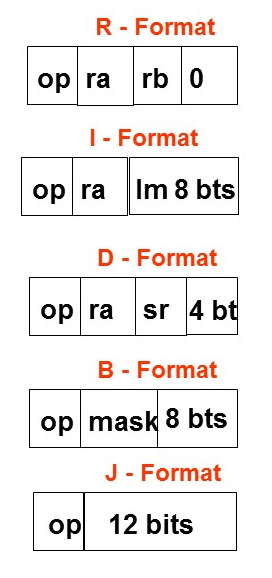
\includegraphics[width=0.2\textwidth]{images/instruction_format.jpg}}
    \caption{UMD-RISC 16 Instruction Modes}
    \label{fig:instruction_format}
  \end{figure}
  \FloatBarrier

% Part 4
  \item Create a testbench to simulate your FPU Entity. When you are ready, integrate both Control and FPU entities together and verify that your design outputs the values you expect in a testbench.

% Part 5
  \item Design a small program (20+ instructions) to test your design using all of the instructions in Table~\ref{tab:riscise} and at least two registers.
  
  A Python assembler is provided to help with generating instructions from assembly to machine code for your design.

	Show that the expected outputs of the FPU are seen at each stage of you testbench in Step 4.

	Document and create a hardware test to run your program. Run all of your instructions and latch the final values of your FPU on a display media of your choice (this includes LEDs, LCD, VGA, etc.). Your final result should be something that builds on each previous instruction to verify your entire program ran as expected.

Show the final hardware test to the professor or TA for verification.
  
\end{enumerate}

\begin{figure}[!htbp]
  \centering
    \begin{Verbatim}[frame=single]
Simple Program:
; In this sample program, the final value would be 2 in R0, a 1 
;   in R5 after all instructions are executed and 4 in R10.

ADDI  R0, 2    ; ADDI R0<-2             R0=2
ADDI  R1, 1    ; ADDI R1<-1             R1=1
SW    R1, $0F  ; DataMem[0F] <- [R1]    DM[0F]=1
LW    R5, $0F  ; R5 <- DataMem[0F]      R5=1
ADD   R0, R5   ; ADD  R0<-R0 + R5       R0=3
AND   R0, R1   ; AND  R0<-R0 & R1       R0=1
OR    R0, R1   ; OR   R0<-R0 or R1      R0=1
ADD   R0, R1   ; ADD  R0<-R0 + R1       R0=2
MOV   R10,R1   ; R10 <- R1              R10=1
SL    R10, 3   ; R10 R10[23:3&000]      R10=8
SR    R10, 1   ; R10 [0& 22:0]          R10=4

The resulting instruction word translation:

5002
5101
A10F
950F
0050
2010
3010
0010
4A10
7A03
8A01
    \end{Verbatim}
  \caption{Program Instruction Example}
  \label{fig:instruction_example}
\end{figure}


\begin{figure}[!htbp]
  \centering
    \fbox{\includegraphics[width=0.5\textwidth]{images/test_configuration.png}}
  \caption{Possible UMD RISC Test configuration}
  \label{fig:test_configuration}
\end{figure}

\section{Deliverables:}

Please only print out your testbench code. A print out of all your code is not necessary. Please zip all VHDL files and UCF file and email to the \textbf{Instructor} and the \textbf{TA} with the filename \textbf{ECE368\_Project\_ Lab1\_Team\#.zip}. Describe your new VHDL designs in your lab report. You can use portions of the code or complete listings if necessary, but discuss how the components operate and any required conditions or constraints on them.

Explain your testbench, print out your testbench results, and discuss the results you observed. Likewise, explain your hardware test fully and discuss any final results and/or problems you encountered. Include any handwritten design flowcharts or pseudocode used in your lab report.

\section{Lab Report:}

Each lab group should prepare a lab report with the following information:
\begin{itemize}
  \item Follow the \textbf{CPE Laboratory Report Guidelines} for base format
  \item Machine RTL block level design
  \item VHDL component specification and schematic designs.
  \item VHDL system specification and resulting schematic design.
  \item Test plan design and test bench code
  \item Hardware test procedure used to verify your design
  \item Simulation results for your simple machine using a testbench (Prove it works).
  \item Schematic and UCF file for your simple machine.
  \item Conclusion needs to include a discussion of the learning utility of this lab and discussion of any issues you had with lab design and clarity.
  \item Reflection section discussing what you did well in your design, what you did not so good and why and what you plan to do to improve your design and design skills in the next lab and for the final project.
\end{itemize}

\begin{figure}[!htbp]
  \centering
    \fbox{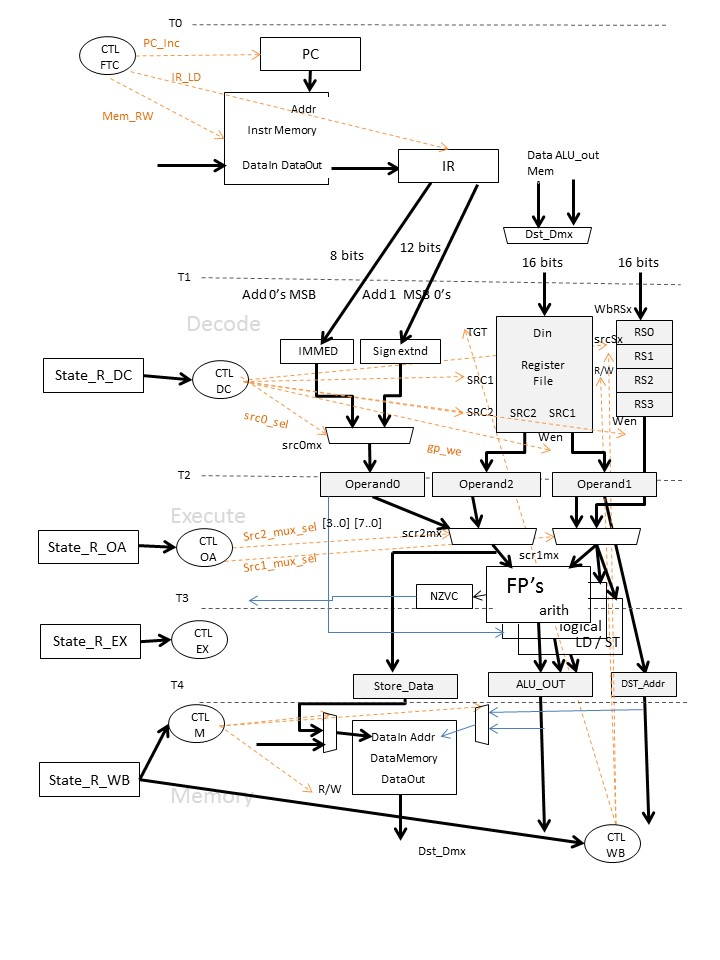
\includegraphics[width=0.8\textwidth]{images/data_control_paths.jpg}}
  \caption{Notional Pipelined Data Path and Control Paths}
  \label{fig:data_control_paths}
\end{figure}
\newpage

\section{Project Lab 1 Grade}

\begin{table}[!htb]
  \begin{center}
    \begin{tabular}[width=0.9\textwidth]{|l|c|l|}
       \hline
       Section & Value & Score\\
       \hline 
       \multicolumn{1}{|l}{\textbf{Procedure:}}  & -\textbf{60}- &\\
       \hline
       1. Design the Control Path Entity & 20 &\\
       \hline
       2. Simulate Control Entity & 10 &\\
       \hline
       3. Design the FPU Entity and associate components & 20 &\\
       \hline
       4. Simulate FPU entity with Control Entity & 5 &\\
       \hline
       5. Show Final Hardware Test & 5 &\\
       \hline
       \multicolumn{1}{|l}{\textbf{Deliverables:}}  & -\textbf{20}- &\\
       \hline
       \multicolumn{1}{|l}{\textbf{Lab Report:}}  & -\textbf{20}- &\\
       \hline
       \hline
       \multicolumn{1}{|l}{Total} & \multicolumn{1}{c|}{100} &\\
       \hline
    \end{tabular}
  \end{center}
  \caption{Project Lab 1 Grade Breakdown}
\end{table}

\end{document}
